\chapter[Theoretical Foundations of Optimal Transport]{Theoretical Foundations of \\Optimal Transport}
\label{ch:2}
Before we can work on the problem at hand, we need to properly define what (inverse) Optimal Transport (OT) is. For this, we will first recap a bit of measure theory. \par 
The theory in this chapter is mainly based on \citet{villani2008}, \citet{benamou1998}, \citet{peyre2020} and \citet{chiu2022}. To shorten this chapter, proofs of some statements are left out, they can be found in the mentioned papers.\par

\section{Measure Theory}
The reader is assumed to be familiar with the basic concepts of measure theory. Here, we will introduce a concept that is helpful to understand the language optimal transport theory is formulated in. We will look at the \textit{coupling} of two measures: 
\vspace{0.3cm}
\begin{definition}[Coupling]
	Let $(X, \mu)$ and $(Y, \nu)$ be two probability spaces. By constructing two random variables $X, Y$ on some probability space $(\Omega, \P)$, $\mu$ and $\nu$ are coupled if $\text{law } (X) = \mu$ and $\text{law }(Y) = \nu$, with the couple $(X,Y)$ being called a \textbf{coupling} of $(\mu, \nu)$. 
	\label{def:coupling}
\end{definition}
Here, law$(X)$ is the probability distribution of $X$. By abuse of terminology, the law of $(X,Y)$ is also called a coupling of $(\mu, \nu)$. \par 
If $\mu$ and $\nu$ are the only laws relevant in the problem, we can assume, without loss of generality, $\Omega = X \times Y$. Hence, coupling $\mu$ and $\nu$ means constructing a measure $\pi$ on $X \times Y$ such that $\pi$ admits $\mu$ and $\nu$ as marginals on $X$ and $Y$ respectively. This measure $\pi$ is what we later define as the transportation matrix. 
\vspace{0.3cm}
\begin{definition}[Deterministic coupling]
	Using the same notation as in Definition~\ref{def:coupling}, a coupling $(X, Y)$ is called \textbf{deterministic} if there exists a measurable function $T: X \ra Y$ such that $Y = T(X)$. 
	\label{def:detcoup}
\end{definition}
This is equivalent to saying one of the following statements: 
\begin{itemize}
	\item $(X,Y)$ is a coupling of $\mu$ and $\nu$ whose law $\pi$ is such that $Y$ can be expressed as a measurable function $T$ on $X$ almost everywhere. 
	\item $X$ has law $\mu$ and $Y = T(X)$ where $T_\#\mu = \nu$, with $\#$ the push forward.
\end{itemize}
In Definition~\ref{def:detcoup}, $T$ is uniquely defined $\mu$-almost surely, and is called the \textbf{transport map}.


\section{Monge-Kantorovich Minimization Problem}
Assume we have a pile of sand and a hole we have to fill with the sand. We can model the sand in both the pile and the hole by probability measures $\mu$ and $\nu$, defined om some measure spaces $X$ and $Y$. Let $A\subseteq X$ and $B\subseteq Y$ be measurable subsets of $X$, respectively $Y$. Then, $\mu(A)$ gives a measure of how much sand is located in $A$ and $\nu(B)$ of how much sand is already in $B$. Moving the sand needs some effort, which can be modeled by a measurable \textit{cost function} $c: X \times Y \ra \R \cup \{+ \infty\}$, where we assume the cost to move sand from $A$ to $B$ can be real-valued or infinite. One can then ask the following question, also known as the mass transport problem: how do we realize the transportation of the sand from $A$ to $B$ at minimal cost? This is the question \citet{monge1781} came up with in his \textit{M\'emoire sur la th\'eorie des d\'eblais et des remblais}, which led to the rise of the theory of optimal transport. \par
\vspace{0.3cm}
\begin{example}[Monge-Kantorovich minimization problem]
	The \textbf{optimal coupling} or \textbf{optimal transport} is a coupling where one introduces a \textbf{cost function} $c(x,y)$ on $X \times Y$, that can be interpreted as the work needed to move one unit of mass from location $x$ to location $y$. Then one considers the \textit{Monge-Kantorovich minimization problem}
	\[\infim_{(\mu, \nu) \sim (X,Y)}\; \E \; c(X,Y), \]
	where the pair $(X,Y)$ runs over all possible couplings of $(\mu, \nu)$, or equivalently
	\begin{equation}
		\infim_{\pi \in \Pi(\mu, \nu)} \int_{X \times Y} c(x,y) d\pi(x,y),
		\label{eq:otdef}
	\end{equation}
	where the infimum runs over all joint probability measures $\pi$ on $X \times Y$ with marginals $\mu$ and $\nu$. Such joint measures are called \textit{transference plans} (or transport plans, or transportation plans), and those achieving the infimum are called \textit{optimal transference plans}. 
	\label{ex:ot}
\end{example}
\vspace{0.3cm}
\begin{remark}
	The transference plans in Example~\ref{ex:ot} are couplings as in Definition~\ref{def:coupling}, and they may be deterministic as in Definition~\ref{def:detcoup}. Hence, the problem of Optimal Transport can be rewritten into the question of looking for a (deterministic) optimal coupling.  
\end{remark}
Now, the problem of finding the optimal transport can be reformulated as follows: let $\rho_0$ and $\rho_T$ be bounded, positive and measurable functions with compact support in $\R^d$. We require they integrate to the same number, which can be normalized to $1$: 
\begin{equation}
	\int_{\R^d} \rho_0(x)\; dx = \int_{\R^d} \rho_T(x) \;  dx = 1. 
	\label{eq:normal}
\end{equation}
We then need to find a mapping, or \textit{application}, $M: \R^d \ra \R^d$ which realizes the transport from $\rho_0$ to $\rho_T$. In other words, we need to find an $M$ for which for all $A \in \mathcal{B}(\R^d)$, there holds 
\begin{equation}
	\int_{M^{-1}(A)} \rho_0(x) \; dx = \int_A \rho_T(x)\; dx.
	\label{eq:benamou2}
\end{equation}
Here, $M$ should be achieving the minimal cost of 
\begin{equation}
	\int_{\R^d} c(x, M(x)) \rho_0(x) \; dx. 
	\label{eq:benamou3}
\end{equation}
Note that the condition in equation~\eqref{eq:benamou2} is equivalent to 
\begin{equation}
	\int_{\R^d} f(M(x)) \rho_0(x) \; dx = \int_{\R^d} f(x)\rho_T(x) \; dx
	\label{eq:equivalence}
\end{equation}
for all continuous functions $f$. 
\vspace{0.3cm}
\begin{example}[Cost function]
	Oftentimes, $\rho_0$ and $\rho_T$ are the initial and final density distributions. Then, equation~\eqref{eq:normal} is the requirement of conservation of mass, and the integrals are all in $\R^3$. \par 
	When $\rho_0$ and $\rho_T$ describe density, the cost function $c$ in equation~\eqref{eq:benamou3} is a function that oftentimes is taken as 
	\begin{equation*}
		c: \R^3 \times \R^3 \ra \R, \;\;\; c(x,y) = ||x - y||^r, \label{eq:benamou4}
	\end{equation*}
	for a certain $r > 0$ (as "cost" should increase by distance), with $||\cdot||$ the Euclidean distance in $\R^3$. \par
	A very common value of $r$ for the cost function is $r=2$ \citep{benamou1998}. This choice is often made because the squared Euclidean distance has applications in fluid dynamics and classical mechanics from the kinetic energy term \citep{benamou2000}. \par 
	Our problem then rewrites to finding the cost function $c: \R^3 \times \R^3 \ra \R$ for which equation~\eqref{eq:benamou3} is being minimized under our observed transport. 
\end{example}

\section{Discrete Optimal Transport}
Now, let us look at discrete OT. For now, let us assume our problem has the same initial and final space, $X = Y = \R^n$. Given a cost matrix $c \in \R^{n\times n}$ with elements $c_{i,j}$, OT as in \eqref{eq:benamou2} can be rewritten as the search for a mapping $M$ in the set $\text{Perm}(n)$ of permutations of $n$ elements while solving 
\begin{equation*}
	\min_{\sigma \in \text{Perm}(n)} \f{1}{n} \sum_{i=1}^n c_{i, \sigma(i)}. 
	\label{eq:optimalmatching}
\end{equation*}
One could naively evaluate this function for all permutations, but the set of all permutations has size $n!$. Hence, for larger datasets, this is not computationally feasible.
\vspace{0.3cm}
\begin{remark}[Uniqueness]
	Note that the optimal transport problem may have several optimal solutions. Consider, for example, $X = Y = \R^2$, with $c$ given as the pairwise distance matrix between the corners of a 2-dimensional square of side length $1$. In that case, only two assignments exists $\sigma = (1, 2)$ or $\sigma = (2, 1)$, and they are both optimal. These assignments can be seen in Figure~\ref{fig:unique}. 
\end{remark}
\vspace{0.3cm}
\begin{example}[Discrete Monge-Kantorovich minimization problem]
	Let $x_1, \dots, x_m \in X$ and $y_1, \dots, y_n \in Y$. Assume we have two discrete measures 
	\begin{equation*}
		\alpha = \sum_{i=1}^m a_i \delta_{x_i} \quad \text{and} \quad \beta = \sum_{j=1}^n b_j \delta_{y_j},
	\end{equation*}
	with weights $a\in \R^m$ and $b \in \R^n$ and positions $x$ and $y$, with $\delta_x$ the Dirac measure at position $x$. Assume all elements of $a$ and $b$ are positive to avoid degeneracy issues. Then, the Monge-Kantovorich minimization problem as in Example~\ref{ex:ot} rewrites to the search for a map $T: \{x_1, \dots, x_m\} \ra \{y_1, \dots, y_n\}$ such that for all $j \in \{1, \dots, n\}$ there holds 
	\[b_j = \sum_{i: T(x_i) = y_j} a_i =: T_\# \alpha. \]
	Note that, since we assumed all elements of $b$ are positive, $T$ is surjective. \par 
	Given a cost $c(x,y)$ defined for certain $(x,y) \in X \times Y$, $T$ should minimize the transportation cost, 
	\[\min_T \left\{ \sum_i c(x_i, T(x_i)): T_\#\alpha = \beta \right\}. \]
	Again, such a map $T$ can be encoded by a permutation $\sigma$. Then, the discrete version of equation~\eqref{eq:benamou2} becomes 
	\begin{equation*}
		\sum_{i \in \sigma^{-1}(j)} a_i = b_j,
	\end{equation*}
	with $\sigma^{-1}(j)$ the pre-image set of $j$. Note that if $m=n$ and $a_i = b_j = 1/n$ (all the weights are uniform), then $T$ is a bijection with $T(x_i) = y_{\sigma(j)}$ and the problem is equivalent to the optimal matching problem \eqref{eq:optimalmatching} with $c_{ij} := c(x_i, y_j)$. 
	\label{ex:discretemonge}
\end{example}
\vspace{0.3cm}
\begin{remark}[Existence]
	Note that a map $T$ as in Example~\ref{ex:discretemonge} may not always exist if $m\neq n$. For example, if $m < n$, the weight vectors are not compatible, and a map $T$ from $\alpha$ to $\beta$ can be found. However, a map from $\beta$ to $\alpha$ cannot be found, since not all elements of $\alpha$ will be reached, and we require $T$ to be surjective.
\end{remark}


\subsection{Solving the Monge-Kantorovich Minimization Problem}
In general, OT can be solved with a linear program. The goal of linear programming is to solve optimization problems with linear objective functions and constraints, which is the case in OT \citep{peyre2020}. In fact, optimal transport problems are equivalent to an important class of linear programs known as cost network flows \citep{korte2018, ford1962}. \par 

% belongs to previous section but here for figure placement 
\begin{figure}[t]
	\centering
	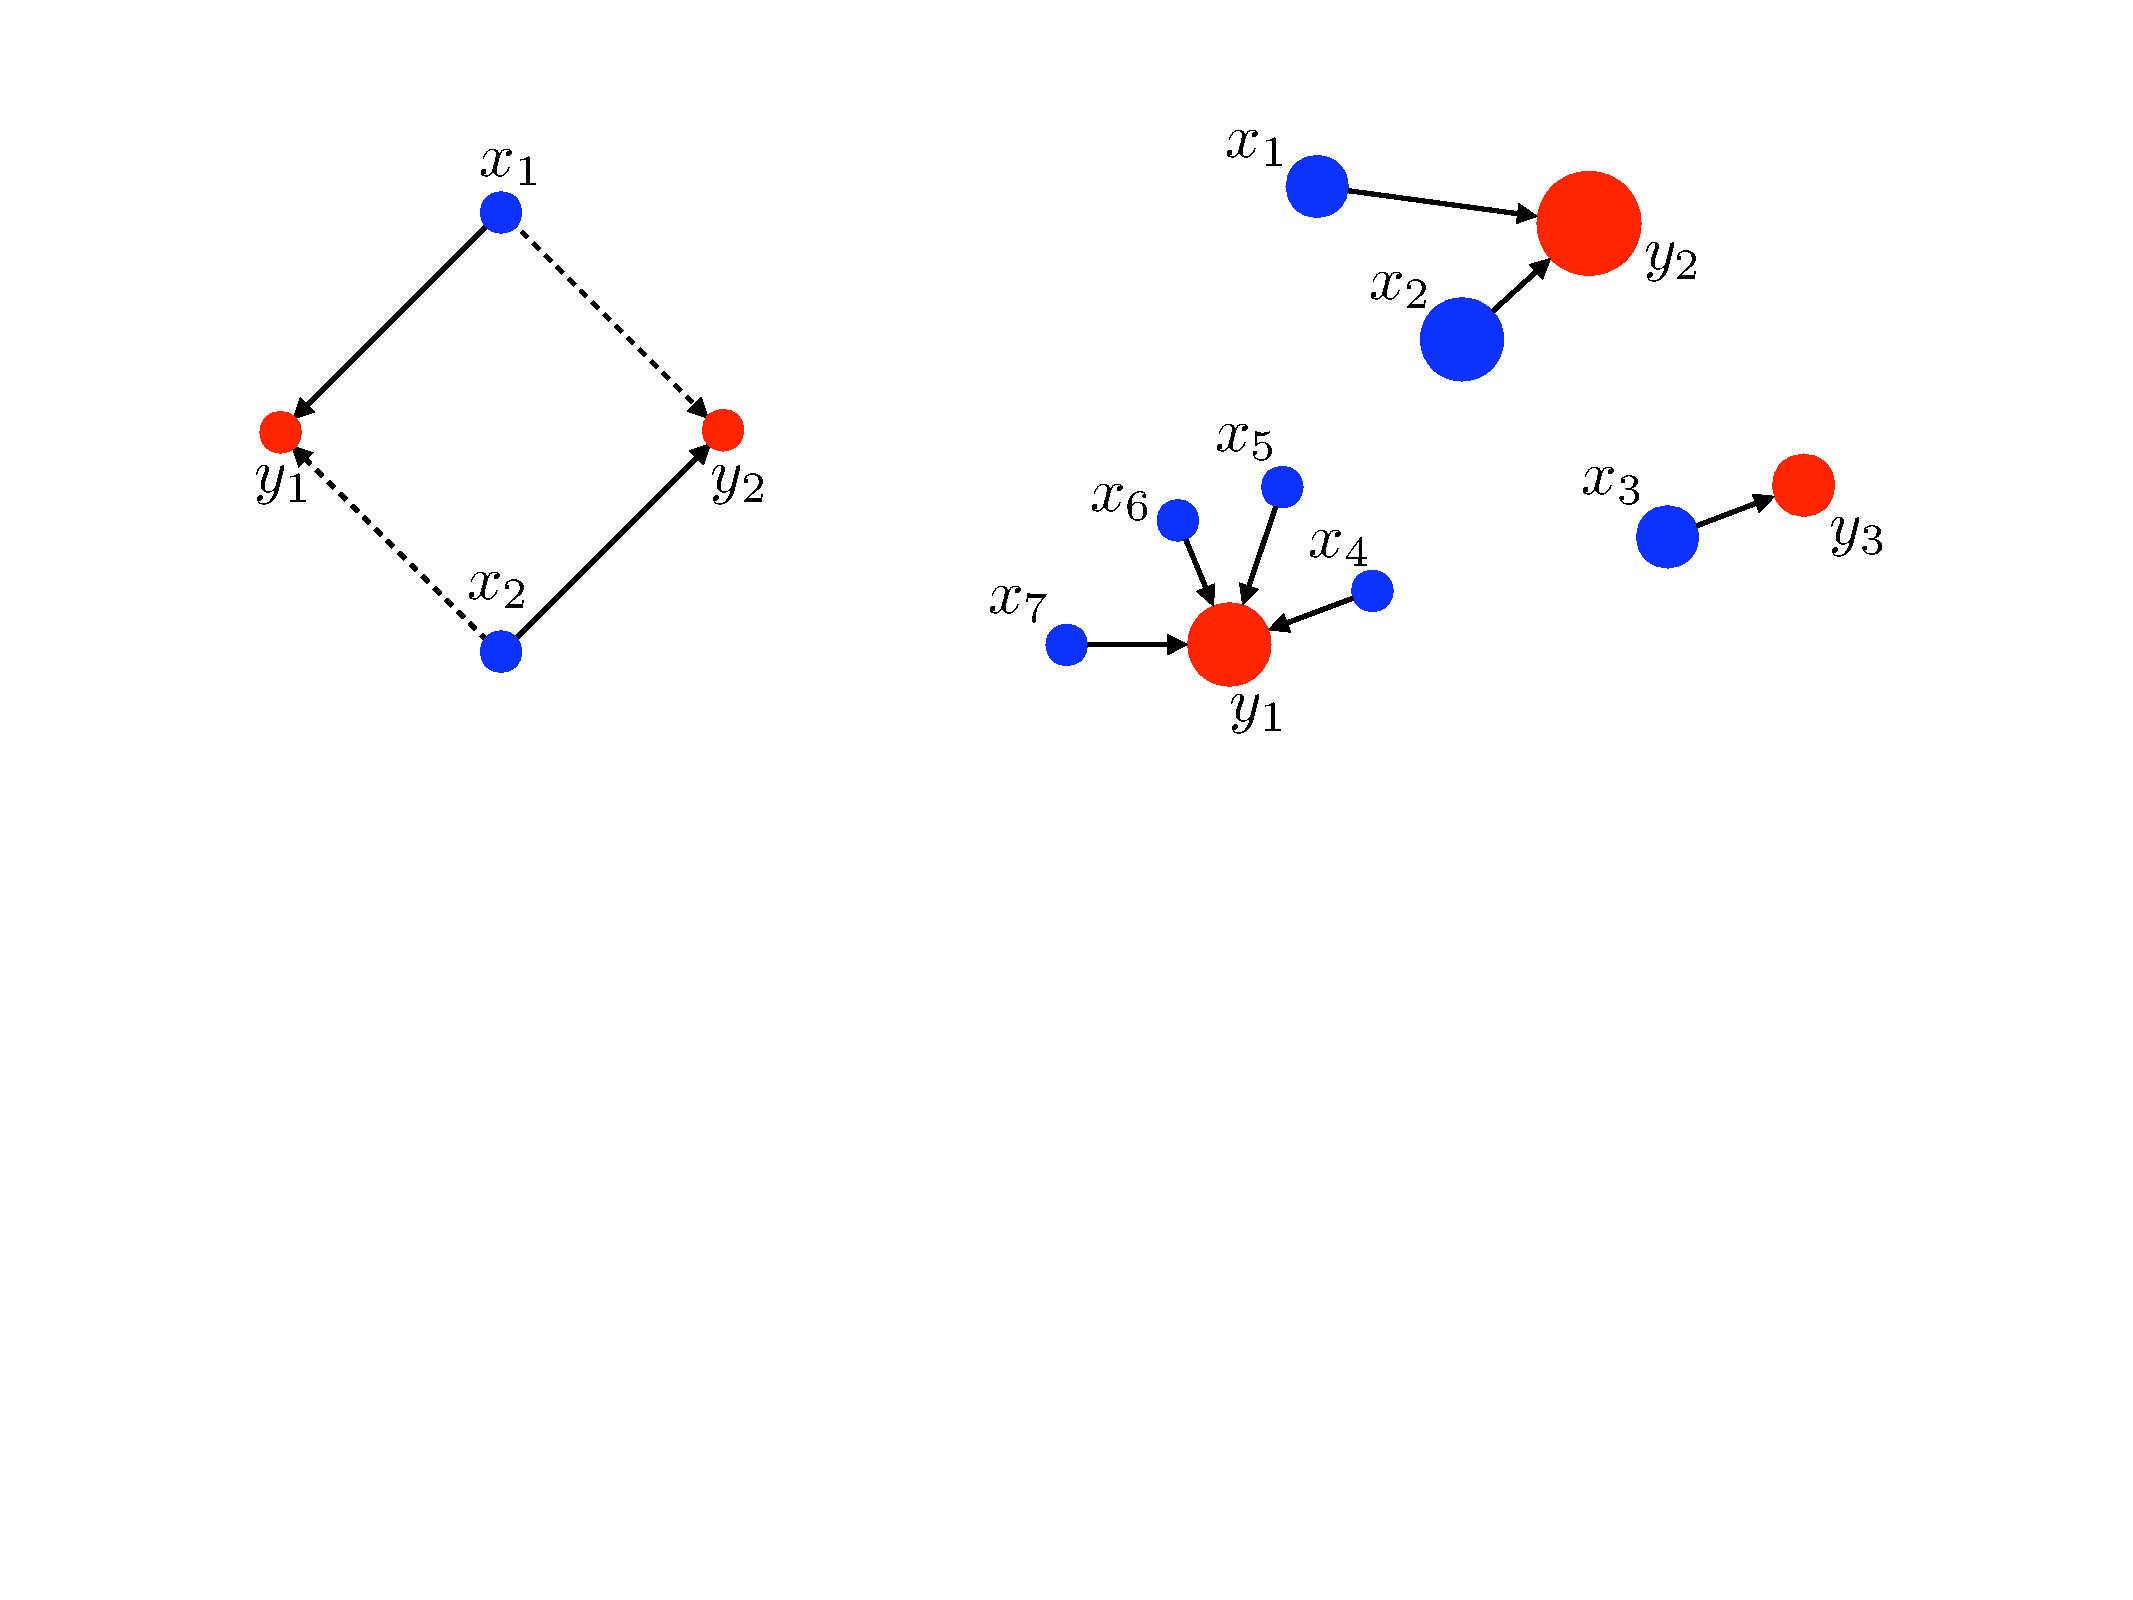
\includegraphics[width=\textwidth]{./images/non-unique-optimal-matching.pdf}
	\caption{\textit{Left}: blue dots from measure $\mu$ and red dots from measure $\nu$. The dots are pairwise equidistant. Hence, either matching $\sigma = (1, 2)$ or $\sigma = (2, 1)$ is optimal.\\ 
		\textit{Right}: a map $T$ can associate measure $\alpha$ to measure $\beta$, with weights proportional to the area of the disk. The mapping is as follows: $T(x_1) = T(x_2) = y_2, T(x_3) = y_3$ and $T(x_4) = T(x_5) = T(x_6) = T(x_7) = x_1$. However, there is no surjective $T$ from $\beta$ to $\alpha$. \\
		Figure 2.2 from \citet{peyre2020}.}
	\label{fig:unique}
\end{figure}

Consider the following OT problem:
\begin{equation}
	\min_{\pi \in \Pi(\alpha, \beta)} \sum_{i = 1}^m \sum_{j = 1}^n c_{ij} \pi_{ij},
	\label{eq:linprog}
\end{equation}
with $\Pi(a,b)$ the set of couplings on $(\alpha, \beta)$ and $c$ a given cost function. One can rewrite equation~\eqref{eq:linprog} into a standard form. Let $\mathbbm{1}_{m \times m}$ be the $m\times m$ identity matrix and let $a \otimes b$ be the Kronecker product. Then, the $(m+n) \times mn$ matrix 
\begin{equation*}
	A = \left[\begin{array}{c}
		\mathbbm{1}_{m \times m}^\top \otimes \mathbbm{1}_{n \times n} \\
		 \mathbbm{1}_{m \times m} \otimes \mathbbm{1}_{n \times n}^\top
	\end{array}\right]
\end{equation*}
can be used to encode the constraints: consider a matrix $P \in \R^{m \times n}$. One can flatten the matrix $P$ onto a vector $p \in \R^{mn}$ by writing $p_{i + m (j-1)} = P_{ij}$. Then, one has \citep{peyre2020}:
\begin{equation*}
	P \in \R^{m \times n} \in \Pi(\mu, \nu) \quad  \Leftrightarrow  \quad p\in \R_{\geq 0}^{mn}, \;\; Ap = \left[\begin{array}{c}
		\mu \\
		\nu
	\end{array}\right].
\end{equation*}
Hence, the original transport problem can be written as 
\begin{align*}
	\min_{p \in \R_{\geq 0}^{mn}} \; c^\top p, \quad \text{such that } Ap = \left[\begin{array}{c}
		\mu \\
		\nu
	\end{array}\right].
\end{align*}
However, note that $p \in \R^{mn}$, so we have $N = mn$ variables. Furthermore, $A$ is a $(m + n) \times mn$ matrix, so we have $K = m + n$ equality constraints. In general, linear programs have a complexity of $\mathcal{O}(N^2K)$ \citep{vanderbei2020}, which is cubic complexity. This can cause issues for large values of $m$ and $n$. 

\section{Entropy Regularization}
\label{sec:entropyreg}
To solve the computational difficulties in OT, \citet{cuturi2013} proposed an entropy regularization of OT. His approach smoothed the classical OT problem with an entropic term, given by
\begin{equation}
	\pi = \argmin_{\pi \in \Pi (\mu, \nu)} \left\{\langle c, \pi \rangle - \varepsilon H(\pi) \right\},
	\label{eq:eotcuturi}
\end{equation}
with $\varepsilon > 0$, $\Pi(\mu, \nu)$ the set of all couplings between $\mu$ and $\nu$, $\langle c, \pi\rangle$ the inner product between $c$ and $\pi$, and 
\begin{equation}
	H(\pi) := -\sum_i \sum_j \pi_{ij} \log \pi_{ij}
	\label{eq:entropyH}
\end{equation}
the entropy of $\pi$, with $\pi$ having entries $\pi_{ij}$. We use the convention $H(\pi) = -\infty$ if one of the entries of $\pi$ is $0$ or negative. The entropy regularized OT solves for the optimal coupling $\pi$ that minimizes the (entropy regularized) cost of transfer from $X$ to $Y$. \par
Note that for $\pi$ a probability matrix, $H$ is strongly concave: $\del^2 H(\pi) = -\text{diag}(1/\pi_{ij})$ and $\pi_{ij} \leq 1$. Therefore, the entropy-regularized problem has a unique solution. \par 
Figure~\ref{fig:impactepsilon} shows the effect of the entropy regularization on the simplex $\Sigma^3$, visualized as a triangle. Note how the entropy term pushes the original linear program solution away from the boundary of the triangle. \par 
\begin{figure}[h!]
	\centering
	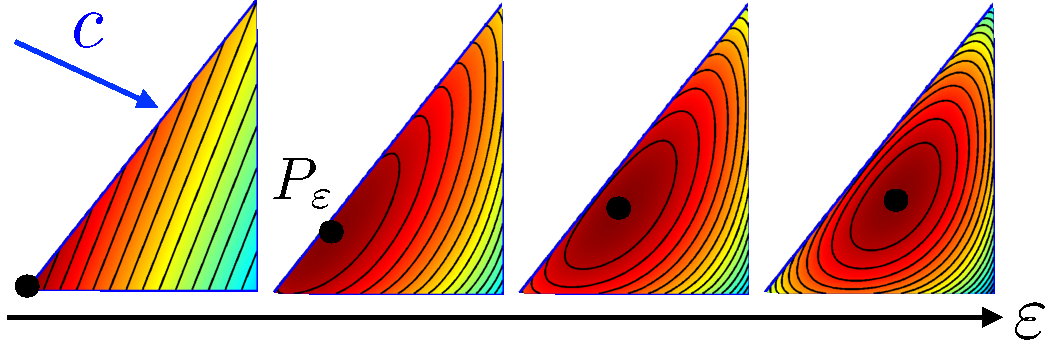
\includegraphics[width=.7\linewidth]{./images/simplex.pdf}
	\caption{Impact of $\varepsilon$ on the optimization of a linear function on the simplex $\Sigma^3$, solving equation~\eqref{eq:eotcuturi} for a varying $\varepsilon$. Figure 4.1 from \citet{peyre2020}. }
	\label{fig:impactepsilon}
\end{figure}
Entropy regularizing OT is helpful, because it takes into account the uncertainty and incompleteness of the data, and it is faster then regular OT. Furthermore, for $\varepsilon \ra 0$, the entropy regularized OT will converge to the regular OT. For $\varepsilon \ra \infty$, the solution converges to the coupling with maximal entropy between the two marginals $\mu$ and $\nu$, $\mu \nu^\top$ \citep{peyre2020}. Thus, as $\varepsilon$ increases, we have faster computational algorithms and statistical convergence. 
	
\subsection{Sinkhorn Scaling}
\label{sec:sinkhorn}
Now, let us look at a specific algorithm for solving equation~\eqref{eq:eotcuturi}. We can define the Kullback-Leibner (KL) divergence between two couplings $\pi$ and $\pihat$ as follows:
\begin{equation}
	\text{KL}(\pihat, \pi) := \sum_{i,j} \pihat_{ij} \log\left(\f{\pihat_{ij}}{\pi_{ij}}\right).
	\label{eq:KLdef}
\end{equation}
Then, the (unique) solution of \eqref{eq:eotcuturi} is a projection onto $\Pi(\mu, \nu)$ of the Gibbs kernel associated to the cost matrix $c$ as 
\begin{equation}
	K_{ij} := \exp\left(-c_{ij}/\varepsilon\right). 
	\label{eq:Kdef}
\end{equation}
After all, when combining \eqref{eq:entropyH} with \eqref{eq:eotcuturi} and using $c_{ij}/\varepsilon = -\log K_{ij}$ from \eqref{eq:Kdef} we get
\begin{align*}
	\min_{\pi \in \Pi(\mu, \nu)}  &\sum_{i,j} \pi_{ij} c_{ij}  + \varepsilon \sum_{ij} \pi_{ij} \log \pi_{ij} \\
	= &\min_{\pi \in \Pi(\mu, \nu)}  \sum_{i,j} \f{\pi_{ij} c_{ij}}{\varepsilon} + \sum_{ij} \pi_{ij} \log \pi_{ij} \\
	= &\min_{\pi \in \Pi(\mu, \nu)} -\sum_{i,j} \pi_{ij} \log K_{ij}  + \sum_{ij} \pi_{ij} \log \pi_{ij} \\
	= &\min_{\pi \in \Pi(\mu, \nu)}  \sum_{i,j} \pi_{ij} \log \f{\pi_{ij}}{K_{ij}}  \\
	= &\;  KL(\pi, K).
\end{align*}
\vspace{0.3cm}
\begin{proposition}
	The solution to \eqref{eq:eotcuturi} is unique and has the form 
	\begin{equation}
		\pi_{ij} = u_i K_{ij} v_j,
		\label{eq:propbenamou}
	\end{equation}
	for $1 \leq i \leq m, 1 \leq j \leq n$ and two scaling variables $u \in \R^m_{\geq 0}, v \in \R^n_{\geq 0}$. 
\end{proposition}
The proof can be found in \citet{peyre2020}, proposition 4.3. \par 
Note that equation~\eqref{eq:propbenamou} can be rewritten as $\pi = \text{diag}(u) K \text{diag}(v)$. Therefore, there must hold 
\begin{equation}
	\text{diag}(u)K\text{diag}(v) \mathbbm{1}_n = \mu \;\;\; \text{and} \;\;\; \text{diag}(v) K^\top \text{diag}(u) \mathbbm{1}_m = \nu.
	\label{eq:ukvdiag}
\end{equation}
Now, note that $\text{diag}(v) \mathbbm{1}_n = v$ and $\text{diag}(u) \mathbbm{1}_m = u$, thus we can see that this is equivalent to 
\begin{equation}
	u \circledast (Kv) = \mu \;\;\;\text{and}\;\;\; v \circledast (K^\top u) = \nu,
	\label{eq:sinkhorn}
\end{equation}
with $\circledast$ the entry-wise multiplication of vectors. This problem is known as the matrix scaling problem \citep{nemirovski1999}. \par 
One way to solve this problem is by Sinkhorn's algorithm \citep{sinkhorn1964}, which can be seen in Algorithm~\ref{alg:sinkhorn}. First we modify $u$ so that it satisfies the left hand side of \eqref{eq:sinkhorn} and then modify $v$ so that it satisfies the right hand side. The updates are then given by 
\begin{equation}
	u^{(l + 1)} := \f{\mu}{Kv^{(l)}} \;\;\; \text{and} \;\;\; v^{(l+1)} := \f{\nu}{K^\top u^{(l+1)}},
\end{equation}
initialized by some arbitrary vector $v^{(0)} \in \R^n$. We stop the iterations when the Euclidean distance $||\cdot||^2$ between the updates of $u$ and $v$ is smaller than some convergence limit $k_u$ and $k_v$ respectively. 
\vspace{0.3cm}
\begin{remark}
	A different initialization will likely end with a different $u$ and $v$, as they are only defined up to a multiplicative constant: if $u$ and $v$ satisfy \eqref{eq:ukvdiag}, then $\lambda u$ and $v/\lambda$ also satisfy \eqref{eq:ukvdiag}, for any $\lambda > 0$. However, these iterations will converge and lead to the same optimal coupling \citep{peyre2020}. Furthermore, note that Algorithm~\ref{alg:sinkhorn} is always convergent for large enough $\varepsilon$. 
\end{remark}
\begin{algorithm}[b]
	\caption{Sinkhorn's Algorithm for OT}
	\textbf{Input: } Cost matrix $c \in \R^{m \times n}$ and regularization parameter $\varepsilon > 0$ and marginals $\mu \in \R^m, \nu \in \R^n$. \\
	\textbf{Initialize:} $v = (1/n, \dots, 1/n) \in \mathbb{R}^{n}$ and $K = \exp(c/\varepsilon)$ \\
	\Repeat{\text{convergent: $||u^{(l)} - u^{(l+1)}||^2 < k_u$ and $||v^{(l)} - v^{(l+1)}||^2 < k_v$}}{
		$u \leftarrow \mu / (K v)$\;
		$v \leftarrow \nu / (K^\top u)$\;
	}
	\KwOut{$\pihat = uKv$}
	\label{alg:sinkhorn}
\end{algorithm}

\vspace{0.3cm}
\begin{example}[Sinkhorn's Algorithm]
	Consider $X = \{x_1, x_2\} = \{1, 3\}$ and $Y = \{y_1, y_2\} = \{2, 4\}$ and two observed probabilities $\mu = (\mu_1, \mu_2) = (1/3, 2/3)$ and $\nu = (\nu_1, \nu_2)= (2/3, 1/3)$. Assume we are given a cost function $c(x,y) = ||x-y||^2$, with $||\cdot||^2$ the Euclidean distance. Then, we can see for the cost matrix:
	\[c = \left(\begin{array}{cc}
		(1-2)^2 & (1-4)^2 \\ 
		(3-2)^2 & (3-4)^2
	\end{array}\right) = \left(\begin{array}{cc}
		1 & 9 \\ 
		1 & 1
	\end{array}\right). \]
	Now, let us investigate Sinkhorn's algorithm. Initialize $v^{0} = (1/2, 1/2)$ and choose $\varepsilon = 0.1$. We can see 
	\[K = e^{-c/\varepsilon} = \left(\begin{array}{cc}
		e^{-1/0.1} & e^{-9/0.1} \\ 
		e^{-1/0.1} & e^{-1/0.1}
	\end{array}\right) \approx \left(\begin{array}{cc}
		4.5 \cdot 10^{-5} & 8.2\cdot 10^{-40} \\ 
		4.5 \cdot 10^{-5} & 4.5 \cdot 10^{-5}
	\end{array}\right).  \]  
	Let us now look at the first iteration: 
	\[u^{(1)} = \f{\mu}{Kv^{(0)}} = \left(\begin{array}{c}
		14684.3 \\ 14684.3 
	\end{array}\right), \quad \text{ and }\quad v^{(1)} := \f{\nu}{K^\top u^{(1)}} = \left(\begin{array}{c}
		0.5 \\ 0.5
	\end{array}\right). \]
	Let us also calculate the second iteration: 
	\[u^{(2)} = \f{\mu}{Kv^{(1)}} = \left(\begin{array}{c}
		14684.3 \\ 14684.3 
	\end{array}\right), \text{ and } v^{(2)} := \f{\nu}{K^\top u^{(2)}} = \left(\begin{array}{c}
		0.5 \\ 0.5
	\end{array}\right). \]
	If we calculate the Frobenius norm, $||\cdot||_F$ of these two iterations, we can see 
	\[ ||u^{(2)} - u^{(1)}||_F \approx 0, \text{ and } ||v^{(2)} - v^{(1)}||_F \approx 0. \]
	This is a very small deviation, and indeed, if we calculate even more iterations, we can see that difference between $u^{(l)}$ and $u^{(l+1)}$ and the difference between $v^{(l)}$ and $v^{(l+1)}$ gets smaller and smaller, thus the algorithm is converging.\par 
	At iteration 20, the difference in $u$ stays down at $0$, as well as the difference in $v$. Calculating the transportation matrix $\pihat$ from this, we get 
	\[ \pihat = u_i v_j K_{ij} \approx \left(\begin{array}{cc}
		0.33 & 6.02 \cdot 10^{-36} \\
		0.33 & 0.33
	\end{array}\right) .  \]
\end{example}

\section{Inverse Optimal Transport}
In some cases, you already know the transportation matrix $\pi$, but you do not know the cost matrix $c$ yet. This case, where you want to solve for $c$, is called \textit{inverse Optimal Transport}, or iOT; it studies the problem of inferring the underlying cost matrix given an observation on coupling two probability measures, such as in transportation. \par 
To solve for the cost function, we will first need to define iOT. However, unlike for the forward problem \citep{villani2008}, the mathematical foundations of the inverse problem have not been intensively studied. Some of the main contributions on iOT are applications of internal migration \citep{stuart2020}, estimating marriage matching \citep{ma2021}, the problem of iOT with noisy and incomplete matching data \citep{li2019}, and the definition on discrete probabilistic iOT \citep{chiu2022}. \par 
To define iOT, let us look at two measurable spaces $X = \{x_1, \dots, x_m\}$ and $Y = \{y_1, \dots, y_n\}$, with $m, n \geq 2$, as the cases where $m=1$ or $n=1$ are trivial. Let $\pi = (\pi_{ij})_{m \times n} \in \R_{\geq 0}^{m \times n}$ be a coupling. Here, $\pi_{ij}$ represents the probability of observing $x_i$ and $y_j$ simultaneously. This interaction can be obtained by a cost matrix $c = (c_{ij})_{m \times n} \in (\R_{\geq 0} \cup \{\infty\})^{m \times n}$, with $c_{ij}$ being the cost of coupling $x_i$ and $y_j$, just as in the forward problem. \par 
Now, given a coupling $\pi$, the inference on $c$ can be formulated as an inverse entropy regularized OT. We know that entropy regularized OT is the map 
\[\Phi: (\R_{\geq 0} \cup \{\infty\})^{m \times n} \times \mathcal{P}(\R^m) \times \mathcal{P}(\R^n) \ra \mathcal{P} (\R_{\geq 0}^{m \times n}), \]
with $\Phi(c, \mu, \nu) = \pi$, $\pi$ as in \eqref{eq:eotcuturi} and $\mathcal{P}(X)$ the set of probability measures on $X$. Then, the inverse entropy regularized OT can be defined as $\Phi^{-1}: \pi \ra \{(c, \mu, \nu)\}$, with $\{(c, \mu, \nu)\}$ the pre-image set of $\pi$ under $\Phi$. 
\vspace{0.3cm}
\begin{remark}
	If $\pi$ is observed without any noise, it completely determines $\mu$ and $\nu$: from $(c, \mu, \nu) \in \Phi^{-1}(\pi)$, we know $\pi \in \Pi(\mu, \nu)$, thus $\mu$ and $\nu$ are the marginals of $\pi$. Thus, we can reduce the problem into $\Phi^{-1}: \pi \ra \{c\}$. However, $\Phi^{-1}: \pi \ra \{c\}$ is not a well-defined function, since $\pi$ does not uniquely determine $c$; for example two cost matrices may differ by an additive constant. 
\end{remark}
Note that we are looking at the entropy regularized OT instead of the regular OT, since the transportation matrix $\pihat$ is in general sparse, and zero elements do not carry enough information to say something meaningful about the cost: a zero in $\pihat$ does not necessarily mean that the underlying cost is infinite \citep{chiu2022}. 





